% !TeX root = ../../thesis.tex
\chapter{Model applications: mechanical integrity of infilled structures}\label{ch:infill}

In this chapter, the developed biodegradation model in chapter \ref{ch:core} is coupled with a level-set based topology optimization procedure that aims to facilitate the design of porous biodegradable scaffolds with complex infill geometries. It's worth mentioning that this chapter is only discussing the first steps of the interaction of these two models rather than a fully developed study. The research presented in this chapter is carried out as an ongoing collaboration work between KU Leuven and Kyoto University, initiated by Dr. Hao Li and Dr. Heng Zhang. The effort put in by Dr. Li for contributing to the code development as well as writing part of this chapter is highly appreciated.

\section{Introduction}

Mg-based alloys are called revolutionary metals in biomedical applications \cite{Shuai2019}, but in order to take advantage of these materials in bone tissue engineering applications, their degradation parameters should be tuned to the bone regeneration rate. One approach to investigating biodegradation behavior is to construct computational models to assess the biodegradation properties prior to conducting any \textit{in vitro} or \textit{in vivo} tests. In addition to degradation tuning, these models can be used for evaluating the mechanical integrity of the implants, which can be considered an important application in bone tissue engineering.

Mechanical integrity can be studied via the change of mechanical properties of the implant over time, an example of which is the stiffness variations of the implant while the degradation takes place. In this chapter, the stiffness change of porous structures during the biodegradation process is investigated by coupling the degradation model and a mechanical analysis model. Such coupling allows studying the correlation of variations in different quantities in both models, such as the effect of mass loss on the structure's compliance and, as a result, on the stiffness.

\newglossaryentry{TO}{name={TO},description={topology optimization}}

Porous (or partially porous) structures are frequently used in biomedical applications due to their attractive properties , one of which is to allow more interaction between the implant and the body environment \cite{Birmingham2012}. A bone implant with a proper lattice structure manufactured with functionally graded materials can improve the healing process of bone defects \cite{Mahmoud2017}. In this chapter, the investigated porous structures are created using a topology optimization (\gls{TO}) routine, in which a set of different volume constraints leads to different final infill shapes.

Performing \gls{TO} on degrading structures has been rarely studied, the reason for which is the difficulty of evaluating the sensitivity of the optimization models in the presence of complex biodegradation mechanisms. Zhang et al. \cite{Zhang2021} presented such a model for a simplified degradation mechanism in which a constant mass loss from the surface was considered in a sophisticated level-set based \gls{TO} to mimic the biodegradation process. In their later work \cite{Zhang2021a}, they enhanced their implementation from the \gls{TO} perspective by extending and verifying it in the microscopic scale for stiffness changeable composite structures. Despite the technical difficulty, the model presented in this chapter can be a first step toward building a coupled model for designing implants by optimizing the structure with the biodegradation tuning taken into account. In this model, the change in the compliance of the degrading structure is calculated in each step of the degradation simulation, making it possible to use it later as the objective function of the \gls{TO} process to consider the effect of biodegradation.


\section{Methods}

The coupled model developed in this chapter includes two sub-models: 1) a level-set-based TO model to get optimized lattice shapes out of initial geometries, and 2) a biodegradation model to perform degradation simulation on the optimized shapes. The computational workflow is such that the TO model generates lattice structures first, which are transferred to the biodegradation model to get the morphology changes due to the degradation process. These morphological changes are then moved to a sub-module of the TO model to compute the change in the strength (stiffness) of the structure and its deformation due to the applied load. A fully-coupled model is still under-development, in which the output of the biodegradation simulation is transferred back to the TO model during the optimization process, making it possible to consider biodegradation as part of the objective function of the optimization routine. Fig. \ref{fig:infill_workflow} shows a schematic representation of how simulation data is being passed from one model to the next, in which the sub-module of the TO model performing the stiffness analysis is depicted as a separate module (component 3) for easier demonstration. The ongoing development is shown in a yellow arrow, indicating that it is not considered in the work presented in this chapter.

\begin{figure}[h]
\centering
\medskip
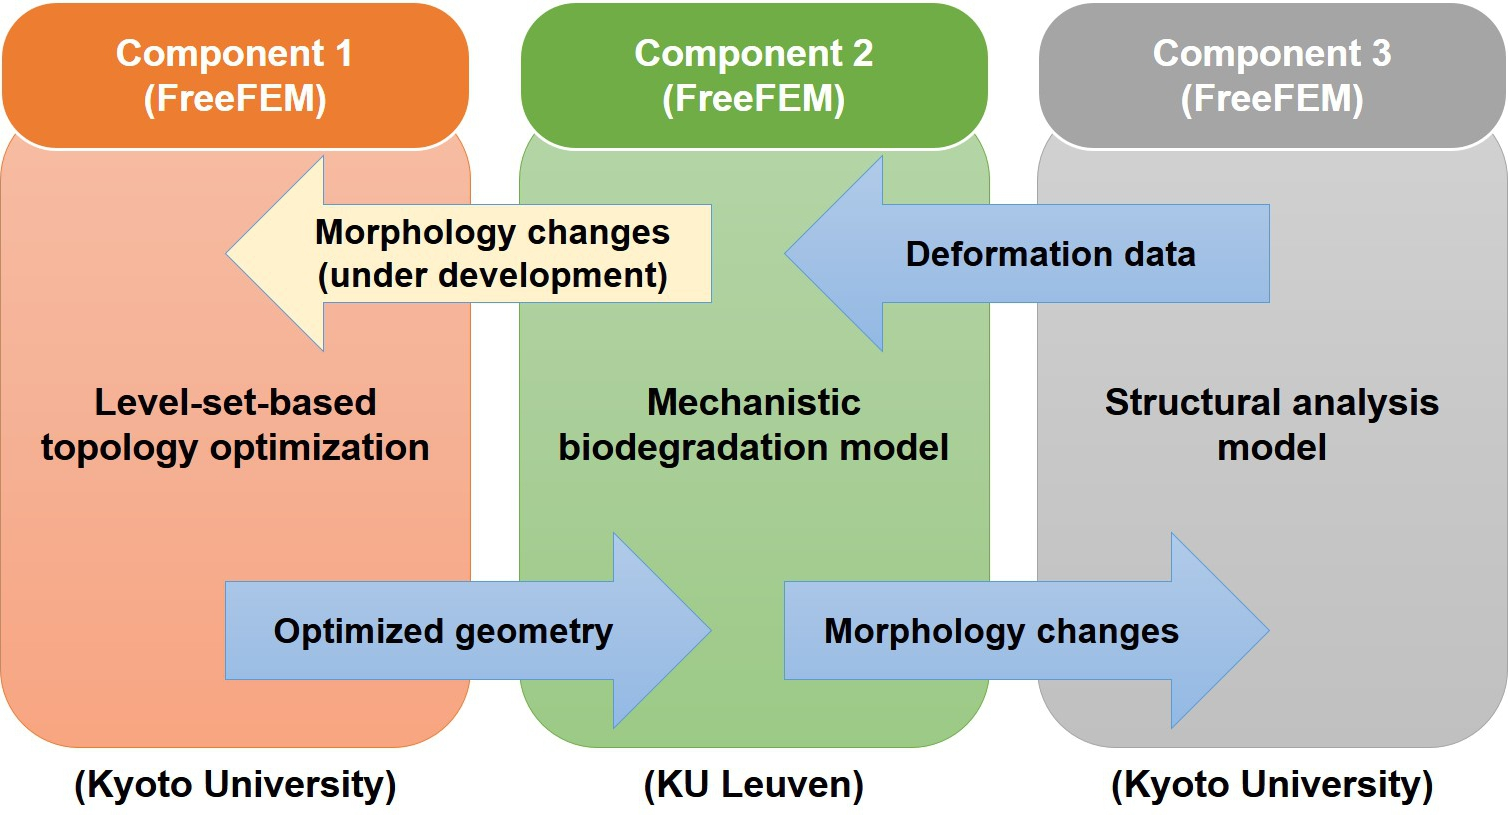
\includegraphics[width=\textwidth]{workflow.jpg}
\caption[Computational workflow of the coupled TO-biodegradation model]{Computational workflow of the coupled TO-biodegradation model, showing how individual components are connected, the programming languages and tools used for the implementation, and the university at which each component is developed.} \label{fig:infill_workflow}
\end{figure}

\subsection{Topology optimization test cases}\label{Section: numerical examples}
In order to prepare the optimized lattices for the biodegradation simulations, the developed \gls{TO} procedure was applied on two 2D test cases, which were different due to type of applied constraint. The details of the developed level-set-based TO is briefly presented in the appendix. The computational domain was a rectangle with a dimension of $2.5L \times 1.0L$. There were two holes inside the domain. The surface traction $\boldsymbol{g}=\left[0,-1\right]^{\operatorname{T}}$ was distributed evenly on the boundary of the right-hand side hole, and that of the left-hand side hole was a fixed wall $\boldsymbol{u}=\left[0,0\right]^{\operatorname{T}}$ (Fig. \ref{fig:infill_domain}). The Young's Modulus was set to $1.0$, and the Poisson's ratio was set to $0.3$. This setup was used for both the TO procedure and the structural analysis used to get the deformations and change of stiffness. For test case \#1, the local volume constraint was imposed, with maximum allowable local volume fraction ($\bar{V}_{\max}$ in Eqs. \ref{eq:infill_vmax_1} and \ref{eq:infill_vmax_2}) set to $0.6$. After being optimized, the global volume fraction was $0.45$. Then, for test case \#2, the global volume constraint was imposed with $V_{\max}=0.45$, the value obtained from the final global volume fraction of test case \#1. The implementation of these numerical examples was done in FreeFEM.

\begin{figure}[h]
\centering
\medskip
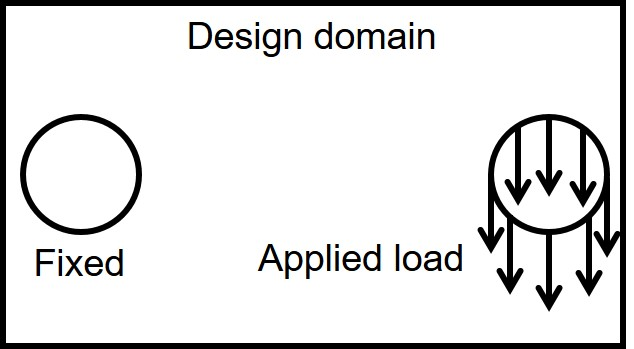
\includegraphics[width=0.5\textwidth]{domain.jpg}
\caption[Computational domain for the topology optimization]{The computational domain used for the topology optimization with the applied load and fixed boundary conditions.} \label{fig:infill_domain}
\end{figure}

\subsection{Biodegradation simulation}\label{section:biodegradation}

The output of the \gls{TO} process for both cases is shown in Fig. \ref{fig:infill_final_cases} (the evolution of the shape to get these lattice structures is discussed later in section \ref{section:infill_results}). Since there is no space surrounding the optimized shapes, this output was embedded in a bigger domain for the biodegradation simulation. For doing this, the output level-set function of the \gls{TO} process was mapped on the mesh of a bigger domain, transforming it into the level-set function of the biodegradation simulation, which is used to track the change in the morphology of the degrading object.

\begin{figure}[h]
\centering
\medskip
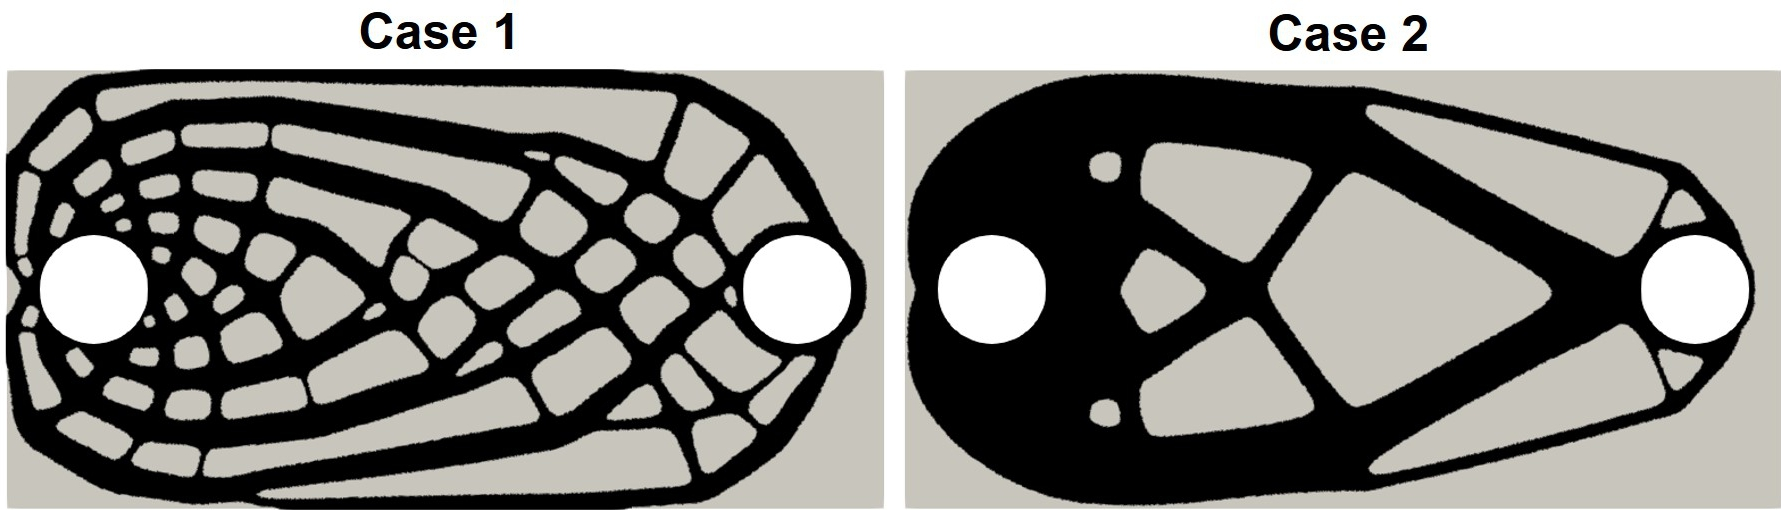
\includegraphics[width=\textwidth]{final_cases.jpg}
\caption[Topology optimization output to be used in the biodegradation simulations]{Topology optimization output to be used in the biodegradation simulations. The black region depicts the optimized material distribution, and the gray zone is the void space. } \label{fig:infill_final_cases}
\end{figure}

The biodegradation simulation was performed using the developed mechanistic model of biodegradation (Chapter \ref{ch:core} and \cite{Barzegari2021}), in which the chemistry of the corrosion process is converted to a set of partial differential equations. The derived \gls{PDE}s are solved using the finite element method implemented in FreeFEM. After mapping the level-set function of the \gls{TO} process to that of the biodegradation model, the computational mesh was refined on the interface of the degrading lattice to increase the accuracy of the interface capturing method, the result of which is demonstrated in Fig. \ref{fig:infill_mesh}.


\begin{figure}[h]
\centering
\medskip
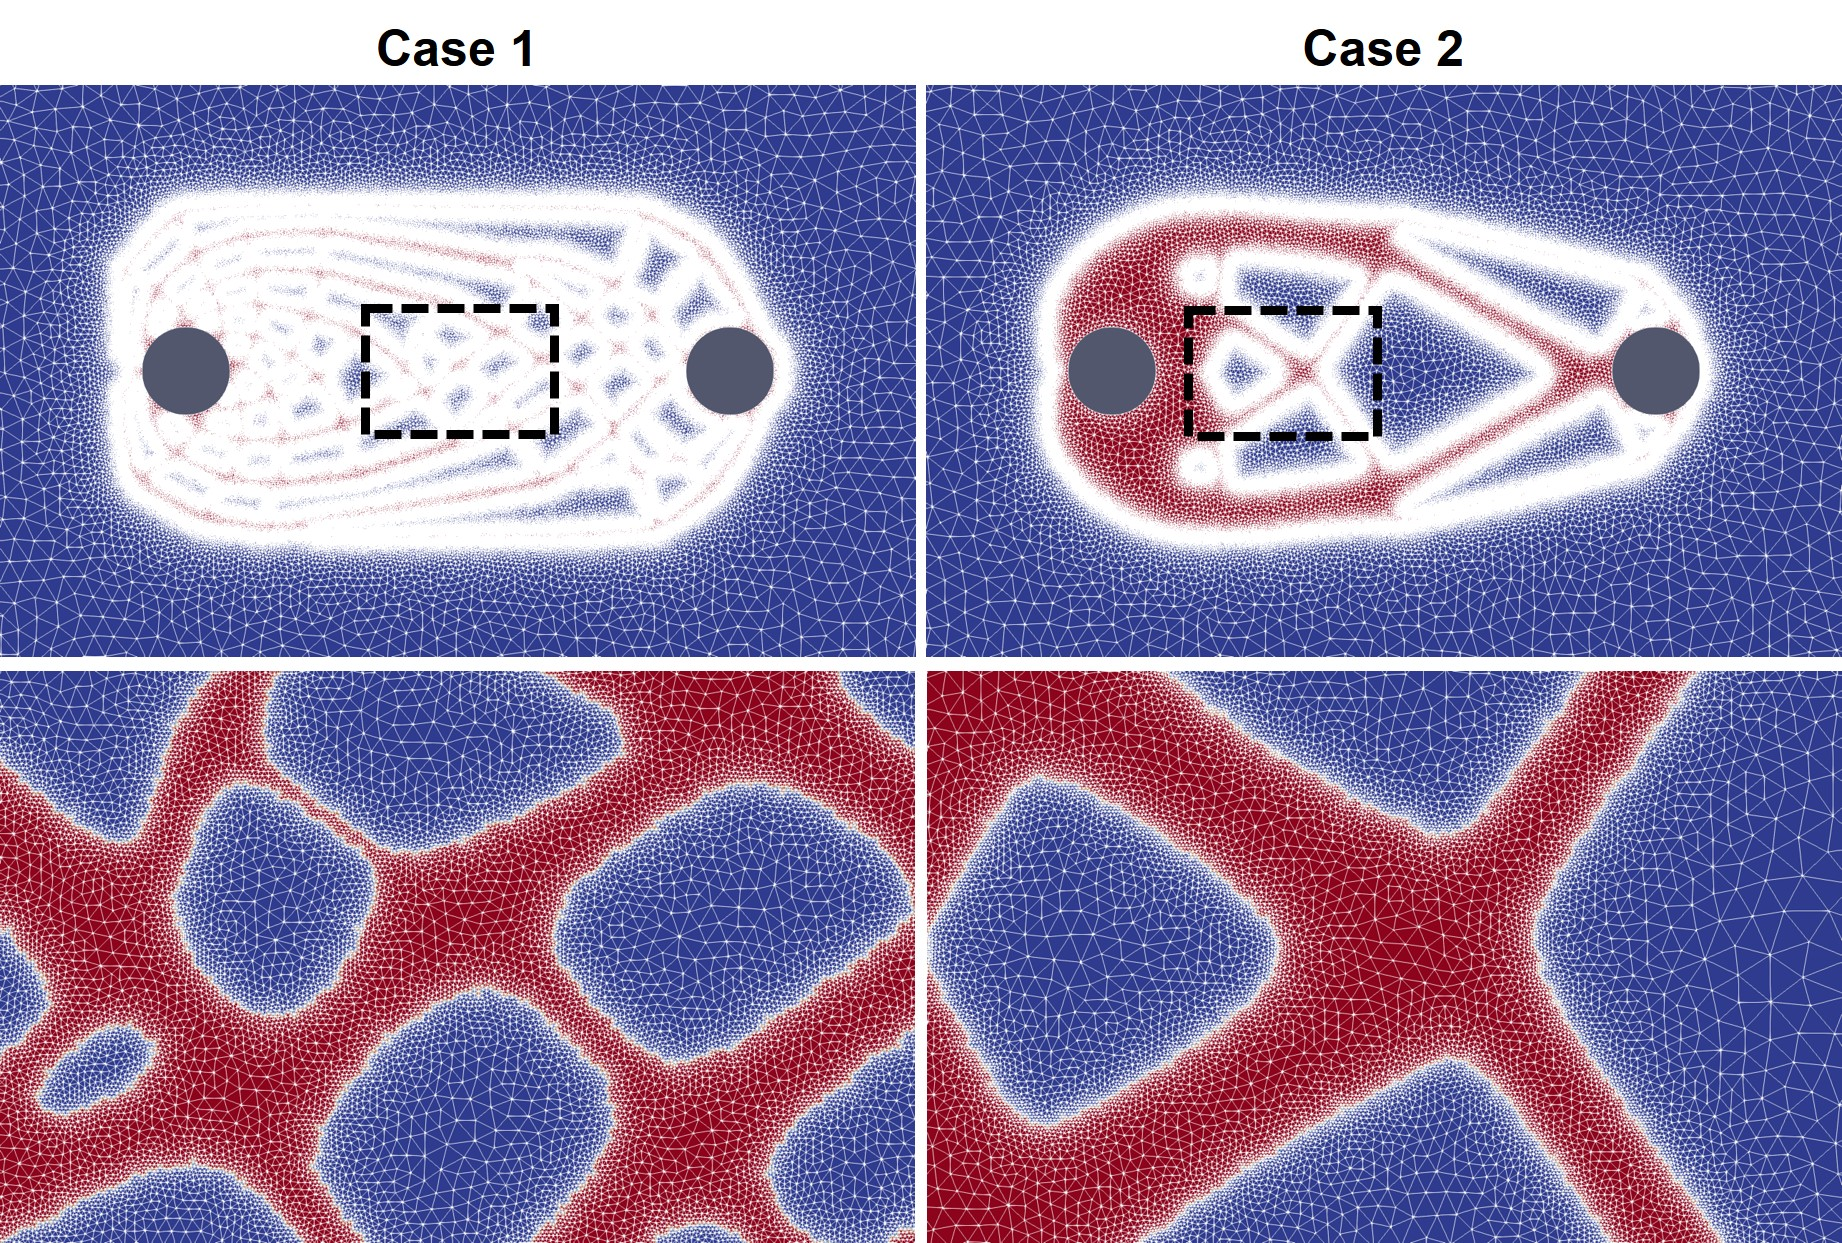
\includegraphics[width=\textwidth]{mesh.jpg}
\caption[Computational mesh for the biodegradation simulations]{Computational mesh for the biodegradation simulations resulted from mapping the \gls{TO} process output to a bigger domain and refining the mesh on the surface of the lattice. The lower row shows the zoomed view of the regions denoted by the dashed rectangle.} \label{fig:infill_mesh}
\end{figure}

The change in the stiffness of the structure was measured during the biodegradation process by applying the boundary condition illustrated in Fig. \ref{fig:infill_domain}. The stiffness was calculated as the inverse of the compliance computed using Eq. \ref{Eq: G'}, which is the sensitivity criterion used for the \gls{TO} process. The biodegradation simulations were performed in three different diffusion regimes (high, low, and medium) in order to investigate the effect of the corrosive environment.



\section{Results and discussion}\label{section:infill_results}

The coupled biodegradation and structural mechanics models were constructed using the output of the \gls{TO} procedure. Fig. \ref{fig:infill_case1_to_steps} shows the temporary evolving shapes of the infilled structures during the optimization process for case 1, each of which is taken by skipping 40 intermediate steps. Fig. \ref{fig:infill_case2_to_steps} shows a similar 2D visualization for case 2. As mentioned in Section \ref{Section: numerical examples}, the difference between these two cases is related to the applied constraints, where a local volume constraint and a global volume constraint were assigned for case 1 and case 2, respectively.


\begin{figure}[h]
\centering
\medskip
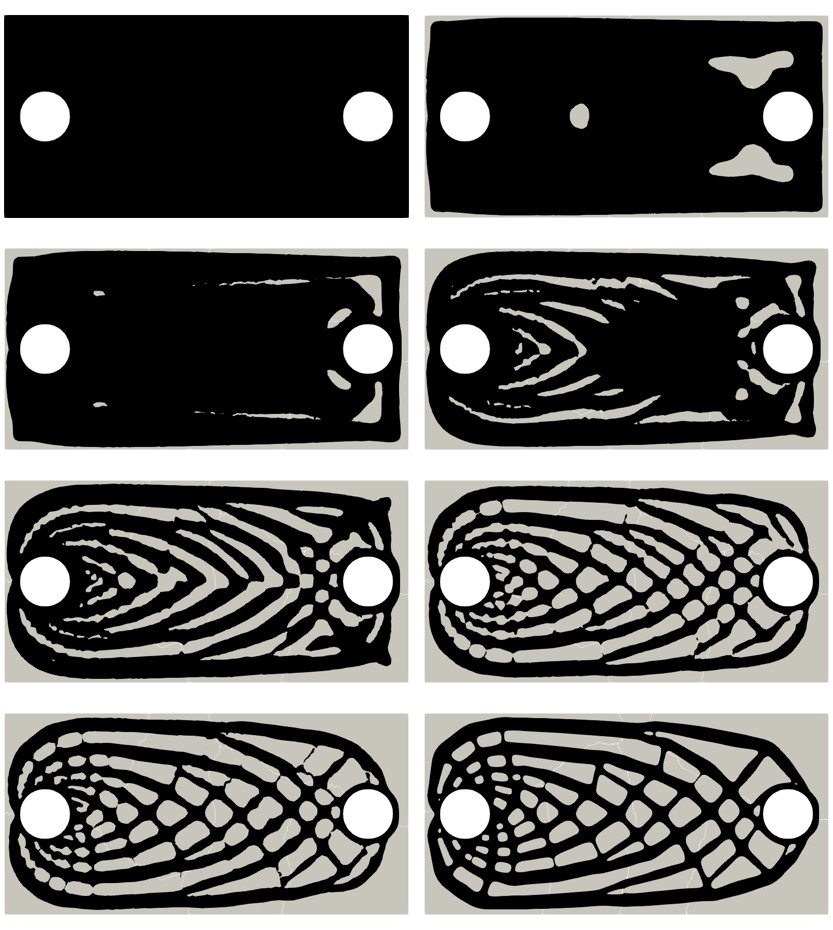
\includegraphics[width=\textwidth]{case1_to_steps.jpg}
\caption[Evolution of the topology optimization level-set function for case 1]{Evolution of the topology optimization level-set function to get the optimized shape for case 1, in which a local volume constraint was imposed.} \label{fig:infill_case1_to_steps}
\end{figure}

\begin{figure}[h]
\centering
\medskip
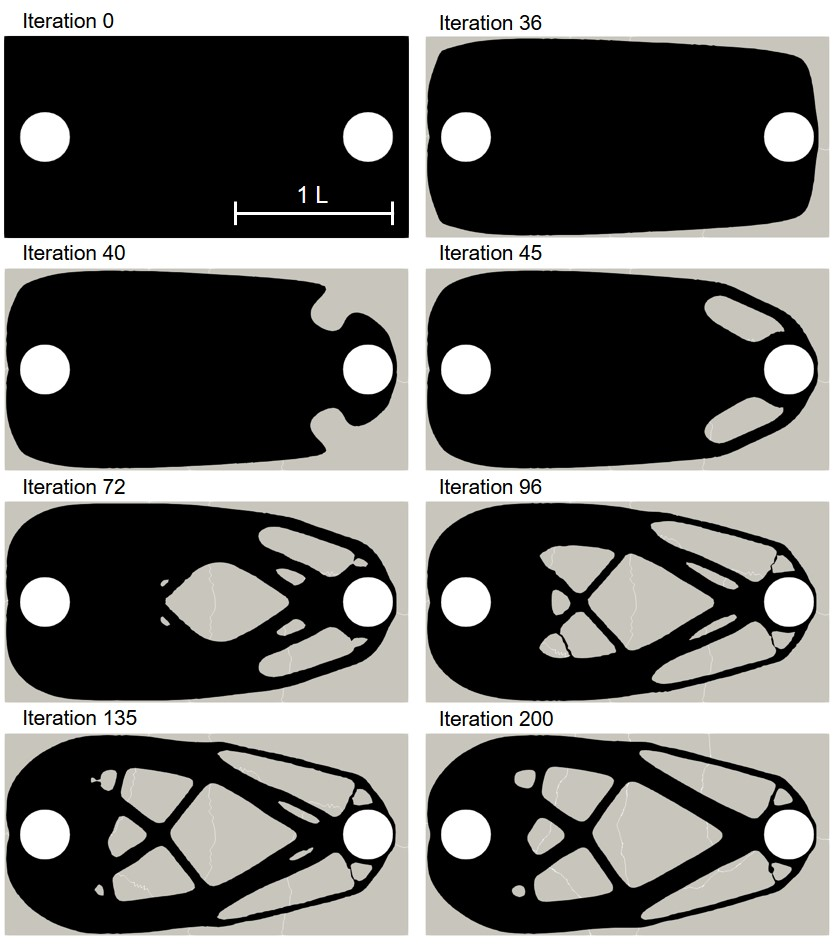
\includegraphics[width=\textwidth]{case2_to_steps.jpg}
\caption[Evolution of the topology optimization level-set function for case 2]{Evolution of the topology optimization level-set function to get the optimized shape for case 2, where only the global volume constraint was imposed.} \label{fig:infill_case2_to_steps}
\end{figure}

Fig. \ref{fig:infill_degradation_stiffness} shows the quantitative results of both components of the coupled computational model for the investigated cases. On the upper row, the degradation rate is plotted by measuring the mass loss over time, showing how the diffusion rate of the Mg ions affects the rate of biodegradation in this model. On the lower row, the change of the stiffness during the biodegradation is plotted, where the stiffness is calculated by inverting the compliance, the objective function of the \gls{TO} routine calculated in each time step after adjusting the geometry in the presence of degradation. The morphology of the object changes as the degradation continues, leading to an increment in compliance and, subsequently, a decrease in the structure's stiffness. This behavior is adequately captured by the coupled model, demonstrating that the models are correctly coupled. Validating the correct predictions of the model on the quantitative effect of degradation on the strength of the structures requires performing further \gls{UQ} analysis to check the sensitivity of the coupled model to chosen parameters.

\begin{figure}[h]
\centering
\medskip
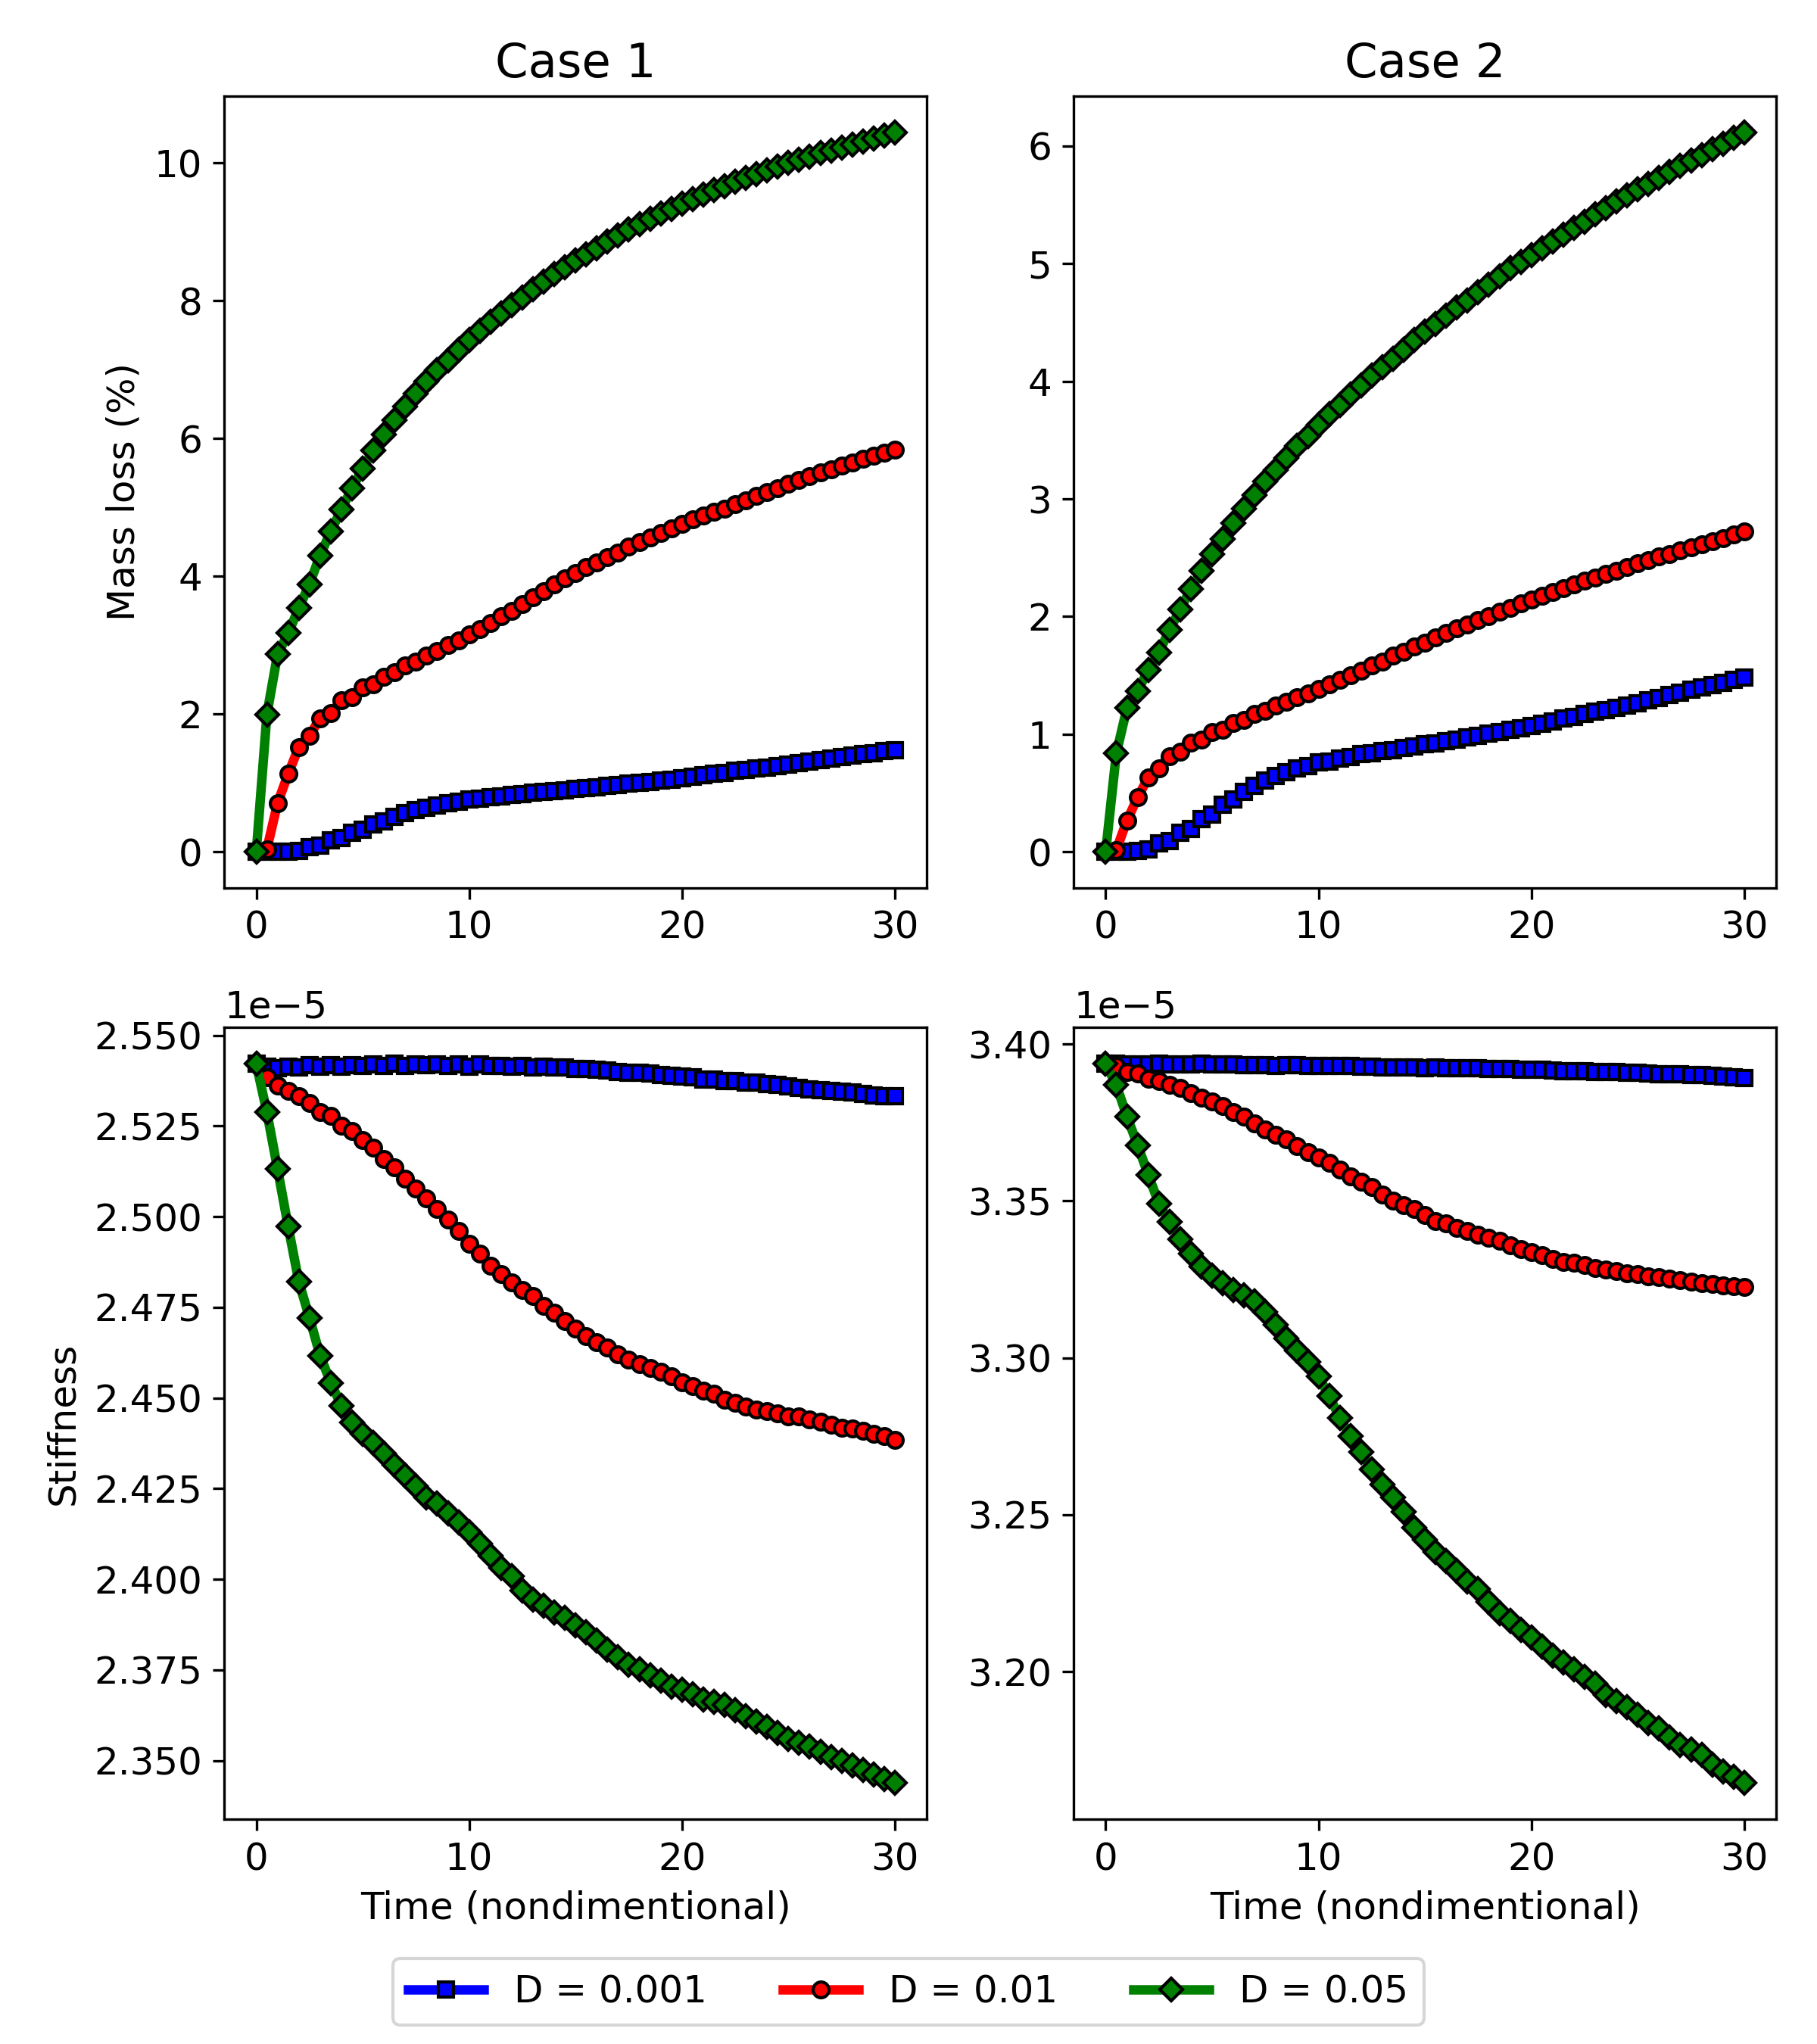
\includegraphics[width=\textwidth]{degradation_stiffness.png}
\caption[Results of the coupled model to predict the stiffness changes during biodegradation]{Results of the coupled model to predict the mass loss and stiffness changes during the biodegradation process of the optimized porous shapes for different Mg diffusion rates. Note the difference in vertical axes scaling.} \label{fig:infill_degradation_stiffness}
\end{figure}

\newglossaryentry{VVUQ}{name={VVUQ},description={verification, validation and uncertainty quantification}}

Case 2 has a higher initial stiffness due to more constitutive materials, but it is also subject to a higher loss of stiffness in the investigated time window compared to case 1 in the high diffusion model (Fig. \ref{fig:infill_degradation_stiffness}). In the first place, this effect may seem to be related to a higher degradation rate and loss of material, i.e., more exposed surfaces to corrosion. However, the mass loss plots show the opposite, where the degradation rate of case 1 is higher in the simulated time window. This observation is more complicated for the medium diffusion regime ($D=0.01$), in which both the drop in stiffness and mass loss are higher for case 1. In low diffusion, both cases show similar behavior. Although not quantitatively validated, these observations demonstrate the necessity of this study, where the mutual effect of biodegradation and the structural characteristics can be investigated to find out the variability of these structural parameters in respect to different degradation parameters. In this study, the effect of only one degradation parameter (diffusion rate) was tested, but the analysis should be further extended by performing sophisticated \gls{VVUQ} analysis on various biodegradation parameters such as the reaction rates. Moreover, the interplay of various parameters can be included in the \gls{TO} process such that the change of morphology of the structure due to biodegradation is taken into account for computing the compliance (TO objective function), yielding more accurate optimization of the morphology of the implants.

Fig. \ref{fig:infill_results_mechanics} demonstrate what the qualitative results of the coupled model look like, in which the infilled part undergoes the degradation and mechanical loading simultaneously. The green surface results from the mechanical analysis, visualized by bending the part according to the computed deformation vector in each node. The light gray surface is the degradation object visualized without bending, showing the change of the morphology due to biodegradation (by comparing the green and gray objects), while the release of the metallic ions is also depicted. The red region shows the release of Mg ions to the surrounding medium, moving the biodegradation interface by shrinkage. This visualization demonstrates the result of the applied boundary condition depicted in Fig. \ref{fig:infill_domain}, where a load is applied to the circumference of the right hole, and the left hole is fixed. These boundary conditions were also used for the \gls{TO} process to get the optimized morphology of the infilled structures.


\begin{figure}[h]
\centering
\medskip
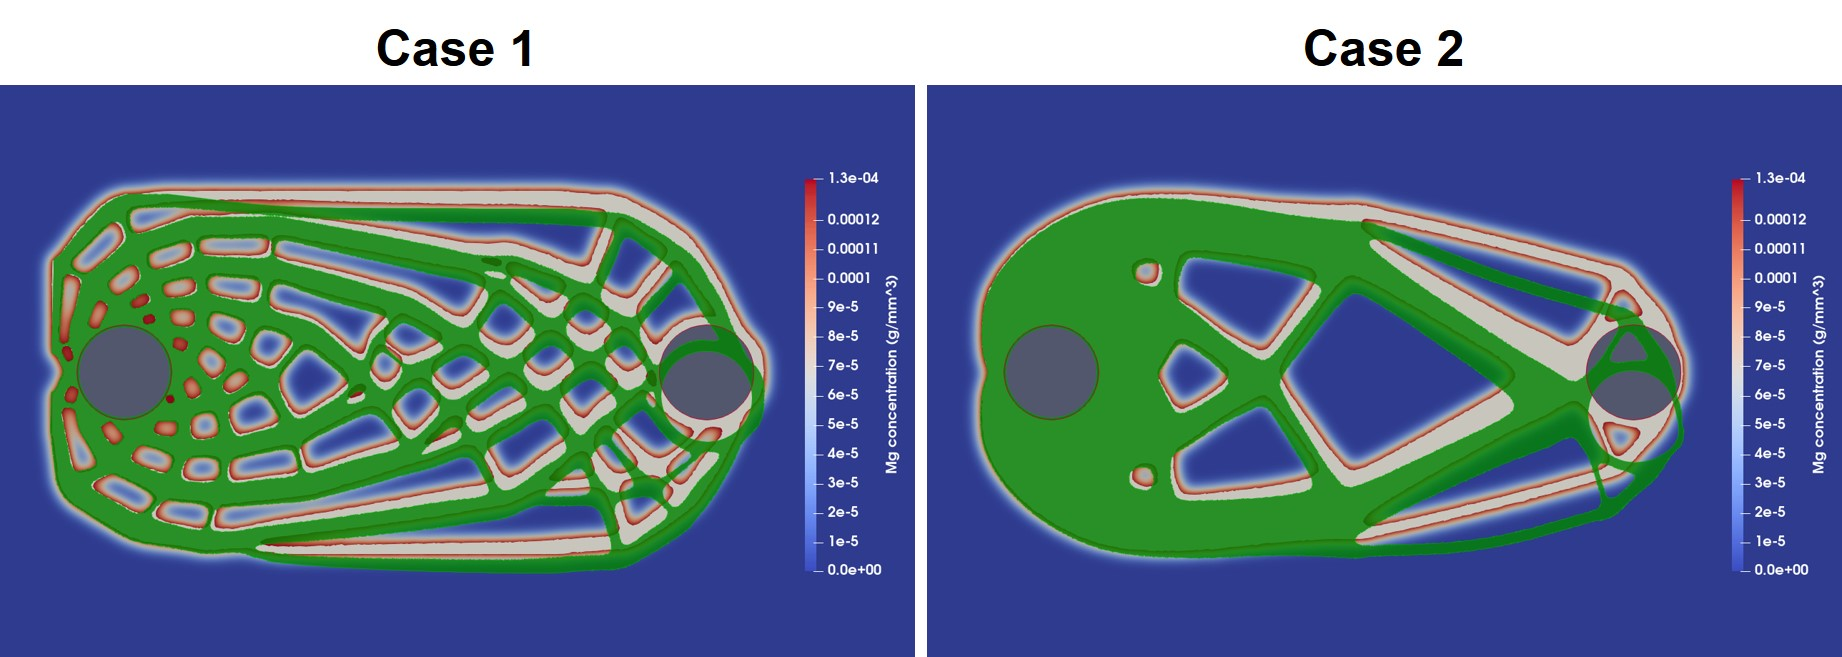
\includegraphics[width=\textwidth]{results_mechanics.jpg}
\caption[Coupled model results showing the structural analysis taking place during biodegradation simulation]{Coupled model results showing the structural analysis taking place during the biodegradation simulation. The green surface shows the deformed infilled structure, and the light gray surface is the state of the morphology during biodegradation. The contour part shows the concentration of metallic ions as being released from the surface of the degrading part.} \label{fig:infill_results_mechanics}
\end{figure}

In order to visualize the biodegradation only, the green surface is removed from Fig. \ref{fig:infill_results_mechanics}, and the results are plotted at various time points during the process. Figs. \ref{fig:infill_results_degradation_case1} and \ref{fig:infill_results_degradation_case2} show such visualization for case 1 and case 2, respectively, showing how the metallic ions are released during the biodegradation process, in which the surface of the degrading part is depicted in light gray. From the biodegradation perspective, the biggest difference between the two studied cases is the exposed surface area, which is higher for case 1, as can be seen in these figures. This fact impacts the degradation rate (Fig. \ref{fig:infill_degradation_stiffness}), leading to a higher loss of material in case 1 in the same simulation time period. However, another crucial aspect to consider is the saturation of the holes disconnected from the bulk electrolyte, where the released materials get accumulate since there is no way for them to spread away. This accumulation prevents further corrosion in the developed biodegradation model because the level-set formulation for the movement of the degradation front works based on the gradient of the concentration of released materials. The absence of gradient caused by the accumulation impacts the rate of degradation, as can be seen in Fig. \ref{fig:infill_degradation_stiffness}, in which the rate of materials loss tends to slow down for case 1. This behavior is more dominant in the high diffusion regime, meaning that the effect can be observed in earlier stages. On the other side, the material loss curve for case 2 shows a semi-linear behavior tending to increase and achieve stability in later stages in comparison to case 1, due to bigger holes in the optimized structure.

\begin{figure}[h]
\centering
\medskip
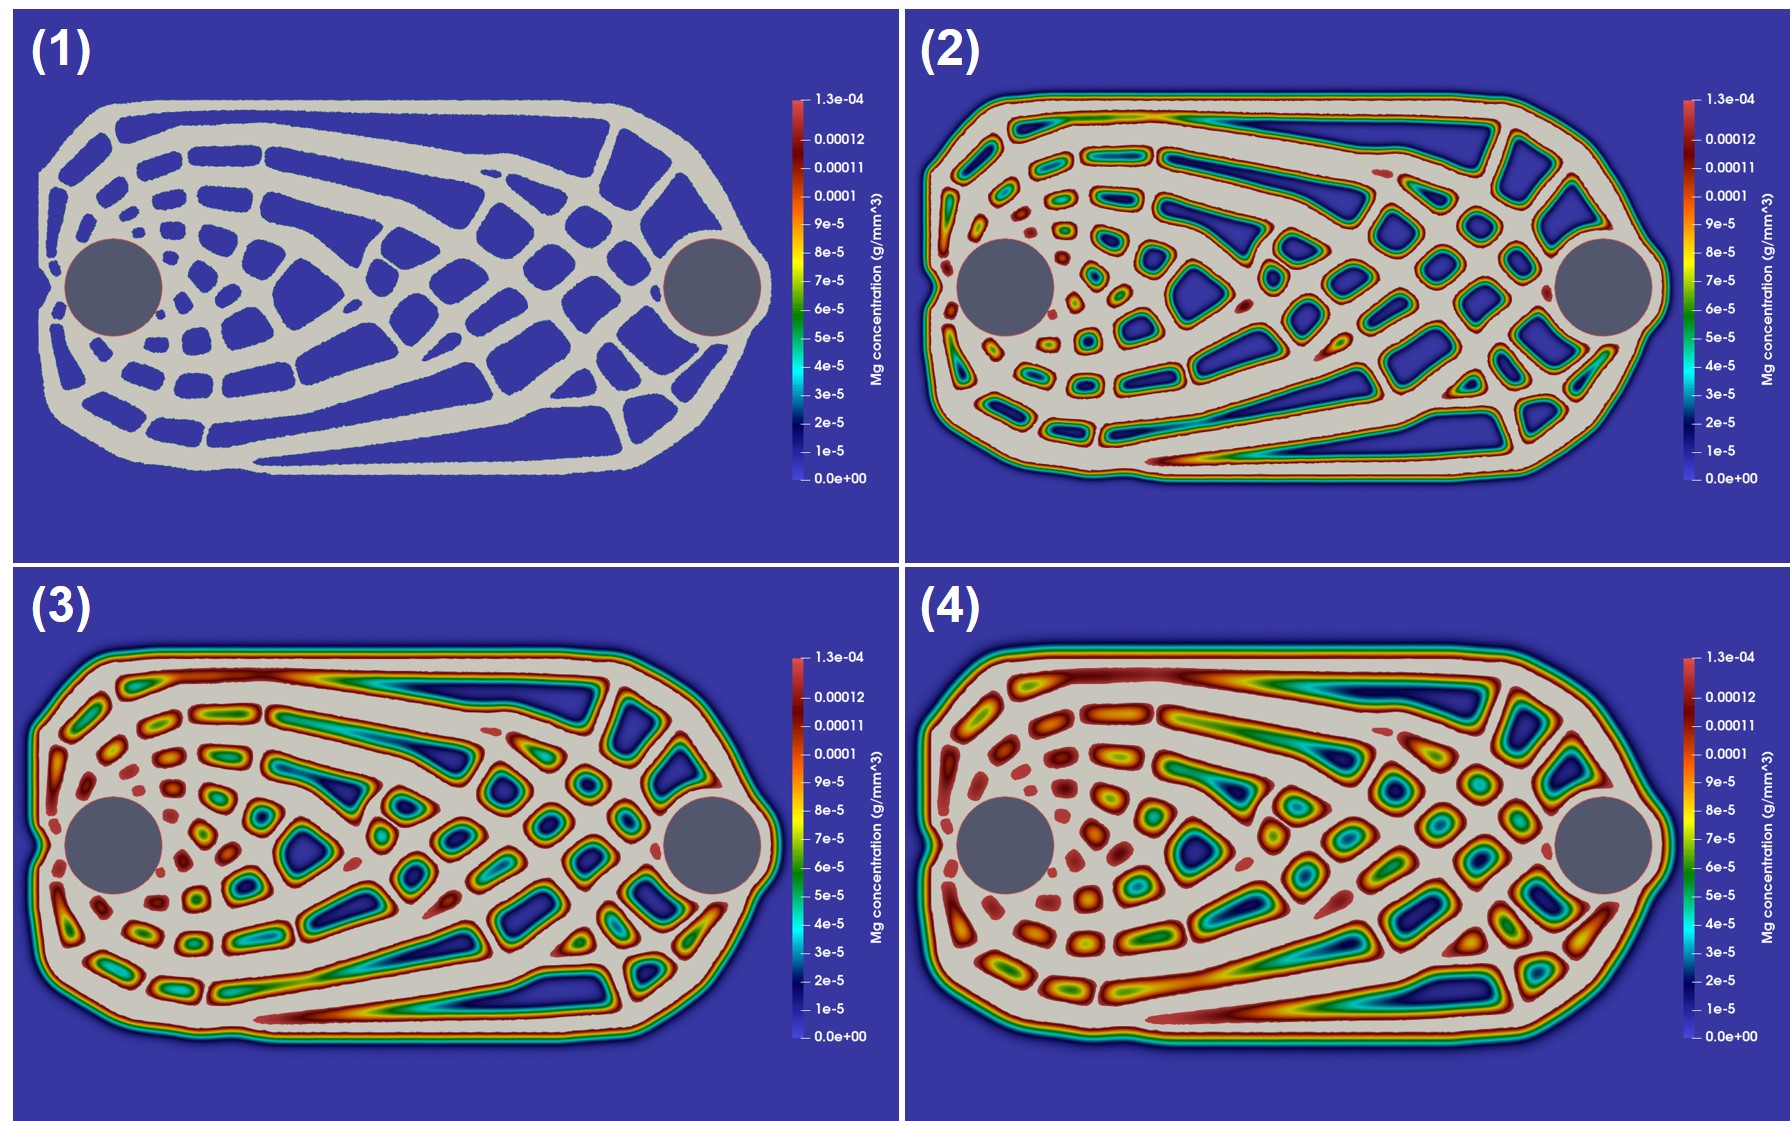
\includegraphics[width=\textwidth]{results_degradation_case1.jpg}
\caption[Visualization of the results of the biodegradation simulation for case 1]{Visualization of the results of the biodegradation simulation for case 1, showing the degradation of the infilled structure and release of Mg ions over time. The colors depict the Mg ions concentration.} \label{fig:infill_results_degradation_case1}
\end{figure}


\begin{figure}[h]
\centering
\medskip
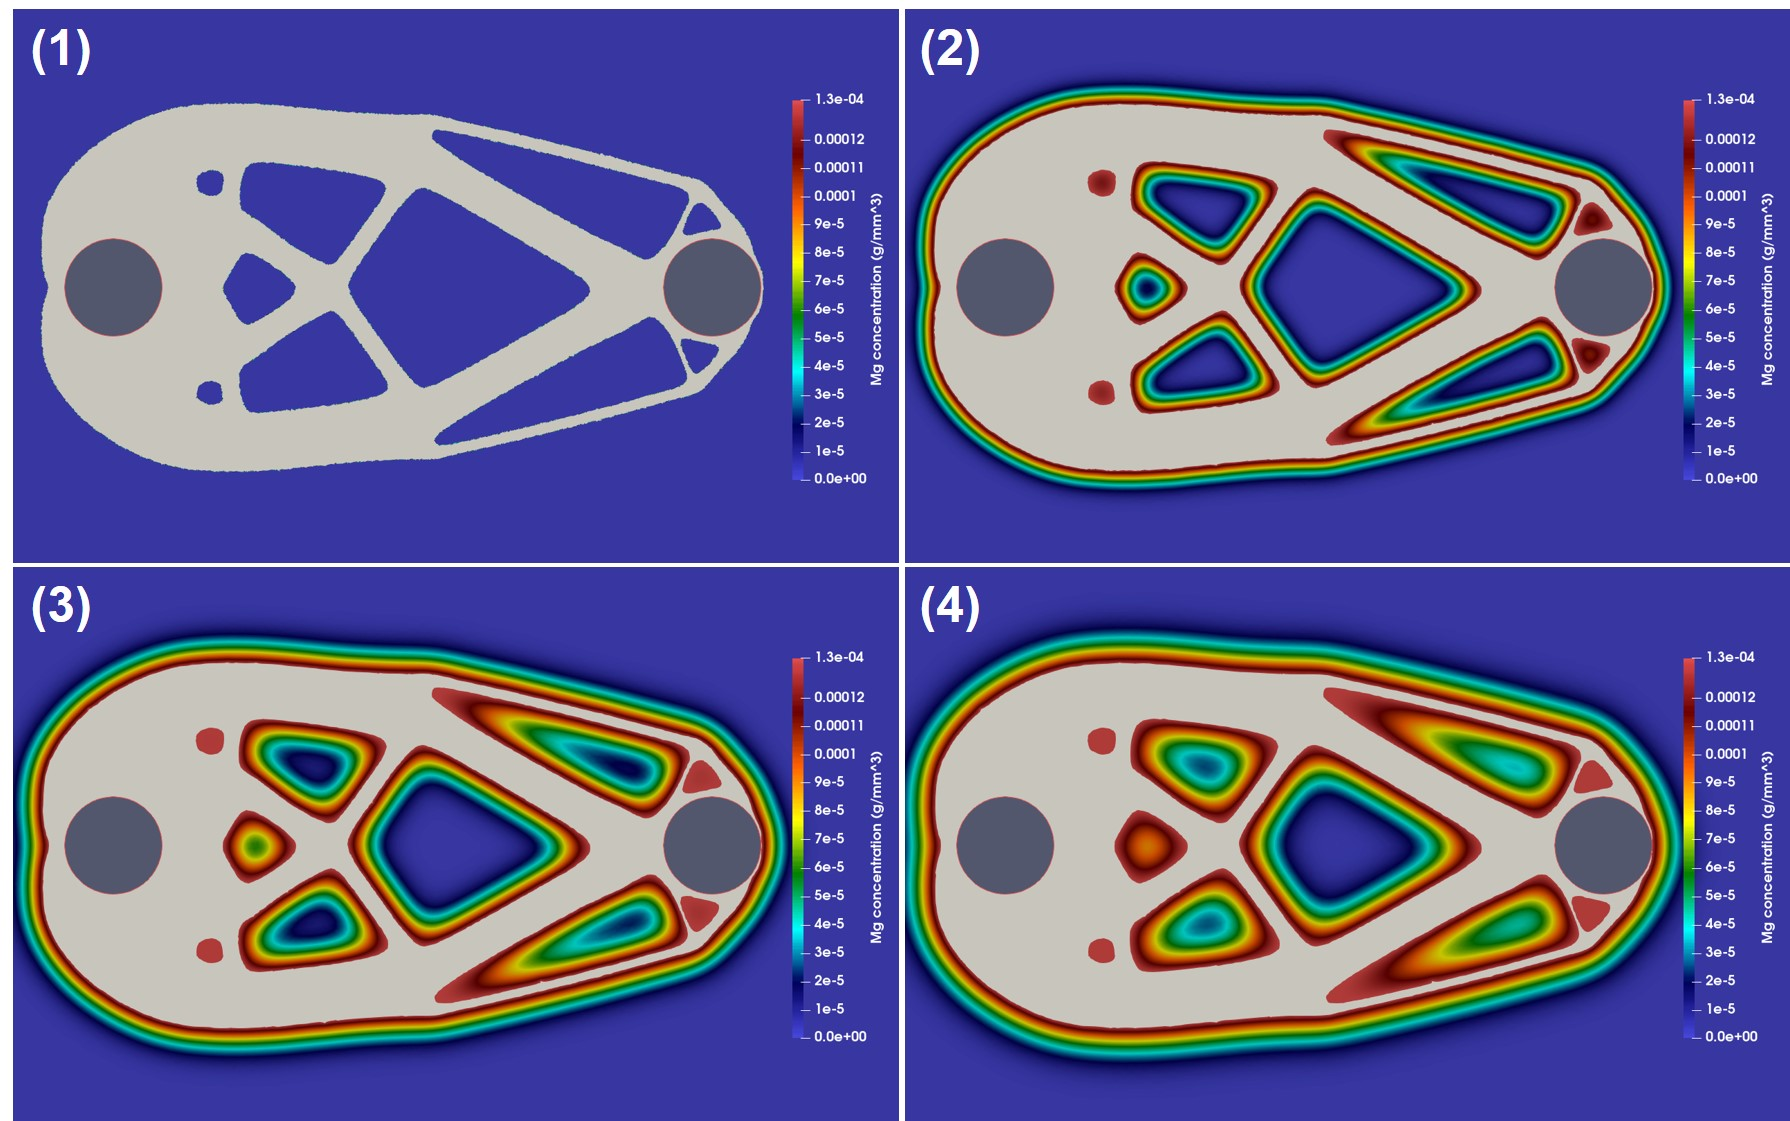
\includegraphics[width=\textwidth]{results_degradation_case2.jpg}
\caption[Visualization of the results of the biodegradation simulation for case 2]{Visualization of the results of the biodegradation simulation for case 2, showing the degrading infilled structure and release of Mg ions over time. The colors depict the Mg ions concentration.} \label{fig:infill_results_degradation_case2}
\end{figure}

It should be noted that the impact of the saturated concentration in the holes is highly dependent on the number of dimensions in $\mathbb{R}^d$, meaning whether it's a 2D or 3D analysis. In a 3D study, the holes have more connections to the bulk volume via the Z axis, whereas in 2D, as in the current study, the isolated holes are the main source of material accumulation which slows down the degradation rate. It emphasizes the necessity of continuing this study by developing a 3D model, which could not be realized in the current stage of model development due to technical difficulties in implementing the parallelization of the coupling techniques. This will be the first consideration in further development of the current coupled model.

As mentioned before, in order to increase the accuracy of the employed interface capturing method, the biodegradation model needs a refined mesh on the metal-environment interface. A closer look at the results of Fig. \ref{fig:infill_results_degradation_case1}, depicted in Fig. \ref{fig:infill_results_degradation_case1_zoom}, shows the mesh being refined on the interface. In this figure, the colors show the concentration of Mg ions released from the interface, and the biodegradation can be observed by the shrinkage of the light gray surface representing the parts of the infilled object that are not degraded yet.


\begin{figure}[h]
\centering
\medskip
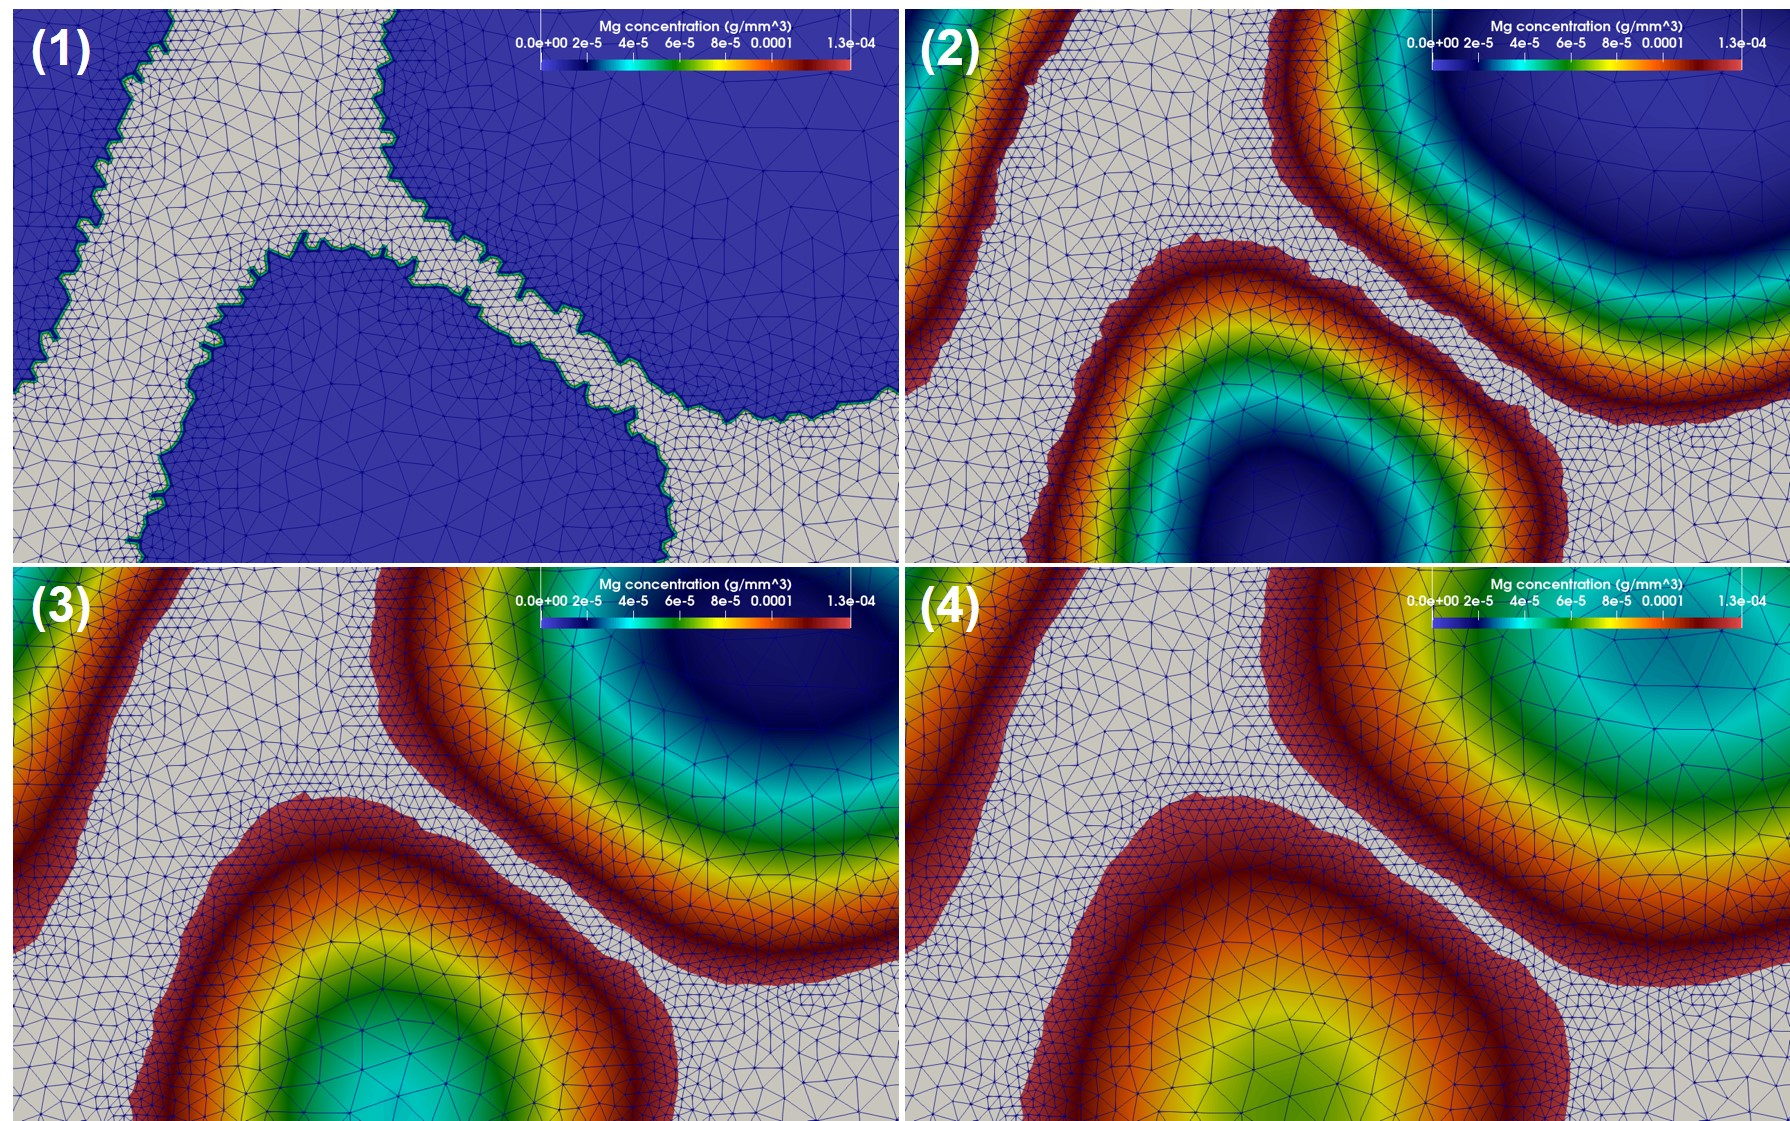
\includegraphics[width=\textwidth]{results_degradation_case1_zoom.jpg}
\caption[Zoom view of the results of the biodegradation simulation for case 1]{Zoomed view of the visualization results of the biodegradation simulation for case 1, showing the refined mesh, the concentration of released ions, and shrinkage of the degrading object.} \label{fig:infill_results_degradation_case1_zoom}
\end{figure}

\section{Conclusion}

In this chapter, the biodegradation model was coupled with a topology optimization code to investigate the effect of biodegradation on the change of mechanical stiffness of porous structures. The development of the proposed coupled model was motivated by the strong desire for biodegradable porous implants for tissue engineering and orthopedic applications. As stated while discussing the results, the reported findings suggest that the biodegradation behavior of these complex structures is not necessarily straightforward to predict without using computer models. As a result, \textit{in silico} studies become crucial to help design the next generation of biomedical implants, in which the structural behavior during the biodegradation process is considered as one of the design objectives.

\begin{subappendices}

\section[Mathematical details of the topology optimization procedure]{Mathematical details of the employed topology optimization procedure}

\newglossaryentry{RDE}{name={RDE},description={reaction-diffusion equation}}

This section provides a brief mathematical summary of the topology optimization of feature-rich structures based on the reaction-diffusion equation-driven (\gls{RDE}-driven) level-set method mostly for readers familiar with TO terminologies and concepts. The reader is encouraged to refer to the PhD work of Hao Li \cite{Li2022Thesis} for elaboration on the employed methodology and implementation.

Section \ref{Section: level-set-based topology optimization method} introduces the basic concept of the \gls{RDE}-driven \gls{TO} method. In section \ref{Section: Maximum length-scale constraint}, the local volume constraint is introduced in this workflow. The key idea here is to use a variational method to compute the local volume fraction, which does not require the spatial information of the adjacent elements. The optimum design problem is formulated in section \ref{Section: topology optimization problem}.


\subsection{Level-set-based topology optimization method}\label{Section: level-set-based topology optimization method}
For the basic concept of the level-set-based \gls{TO} method, we followed the work of Yamada et al.\ \cite{yamada2010topology}. A structural topology optimization problem can be replaced by an optimum design problem to find the optimal material distribution. In other words, this technique essentially answers the question of where the material should be placed or where the hole should be nucleated. Let the computational domain be denoted as $\Omega \subset \mathbb{R}^d$, where $d=2$. A solid subdomain is then defined as $\Omega_{s} \subseteq \Omega$ so that a void domain is as the complementary domain $\Omega \backslash \Omega_{s}$. An implicit level-set function $\phi \left(\boldsymbol{x}\right)$ can be defined to have a piecewise profile as
\begin{equation}
	\left\{\begin{array}{ll}
		{0<\phi(\boldsymbol{x}) \leq 1} & {\text { for } \boldsymbol{x} \in \Omega_{s} \backslash \partial \Omega_{s}} \\
		{\phi(\boldsymbol{x})=0} & {\text { for } \boldsymbol{x} \in \partial \Omega_{s}} \\
		{-1 \leq \phi(\boldsymbol{x})<0} & {\text { for } \boldsymbol{x} \in \Omega \backslash \Omega_{s}},
	\end{array}\right.
\end{equation}
in which the solid--void interface $\partial \Omega_{s}$ can be represented by the zero level-set iso-surface.

Next, using a Heaviside step function, the material field can be modeled using a ``1/0 binary structure'' by the projection of the level-set function $\phi(\mathbf{x})$ to the characteristic function $\chi_{\phi}$ as
\begin{equation}
	\chi_{\phi} :=\left\{\begin{array}{ll}
		{1} & {\text { for } \phi\left( \boldsymbol{x} \right) \geq 0} \\
		{0} & {\text { for } \phi\left( \boldsymbol{x} \right)<0}.
		\label{eq: characteristic function}
	\end{array}\right.
\end{equation}
Using the Ersatz material approach, the material properties inside the computational domain $\Omega$ can be expanded using the obtained $\chi_{\phi}$. The level-set function is obtained as the solution of a reaction--diffusion equation, which can be semi-discretized in a fictitious time-step $\Delta t$, as follows:
\begin{equation}
	\left\{\begin{array}{ll}
		\dfrac{1}{\Delta t} \left( \phi_{n+1} - \phi_{n} \right) =- \left( \tilde{C} \mathcal{F}' -\tau \nabla^{2} \phi_{n+1} \right) & \text{in }\Omega\\
		\nabla \phi \cdot \boldsymbol{n} = 0 & \text{on } \partial\Omega, \\
	\end{array}\right.
	\label{eq: reaction diffusion equation semi discretize}
\end{equation}
where $\boldsymbol{n}$ is the unit normal vector, $\mathcal{F}'$ is the topological design sensitivity, $\tilde{C}$ is the normalizer for the sensitivity, and $\tau$ is the regularization parameter, which can be used to control the complexity of the optimal configuration. The subscript $n$ indicates the fictitious time step. For more details, the reader is referred to the work of Li et al. \cite{li2021full}.

\subsection{Maximum length-scale constraint}\label{Section: Maximum length-scale constraint}
A geometrical constraint is introduced to generate feature-rich structures observed in a natural system such as the trabecular bone. Here, we adopt the idea of Wu et al.\ \cite{wu2017infill} by imposing a maximum allowable volume fraction to the local averaged value of the characteristic function, $\bar{\chi}$. To approximate the maximum value of $\bar{\chi}_i$, we use the $p$-norm function as
\begin{equation} \label{eq:infill_vmax_1}
\max_{\forall i} \left(\bar{\chi}_i \right) \approx
\|\bar{\chi}_i \|_{p}=\left(\sum_i^n \bar{\chi}_{i}^{p}\right)^{1/p}
\leq \left( \sum_{i}^n \bar{V}_{\max}^p \right)^{1/p},
\end{equation}
which can be rewritten as
\begin{equation} \label{eq:infill_vmax_2}
\left(\dfrac{1}{n} \sum_{i} \bar{\chi}_{i}^{p}\right)^{1 / p} \leq \bar{V}_{\max },
\end{equation}
where $n$ is the total number of vertices and $p=10$ in this chapter \cite{li2021full}. Note that in FreeFEM \cite{Hecht2012}, the software package used to solve the derived system, the design variable, i.e. the characteristic function, is defined on the nodes of each element. $ \bar{V}_{\max }$ is the maximum allowable local volume fraction.

Then, we use a \gls{PDE}-filter\ \cite{lazarov2011filters,kawamoto2011heaviside} to compute the local average value $\bar{\chi}$, as
\begin{equation}
	\left\{\begin{aligned}
		& -r^2 \nabla^2 \bar{\chi} +  \bar{\chi} =  \chi & \text{ in } \Omega \\
		& \nabla \bar{\chi} \cdot \boldsymbol{n} = 0 & \text{ on } \partial \Omega,
	\end{aligned}\right.
	\label{Eq: pde filter}
\end{equation}
where $r$ is the filter radius. To clarify the concept of the aforementioned functions, Fig. \ref{fig:infill_diagram} depicts the level-set ($\phi$), characteristic ($\chi$), and local average characteristic ($\bar{\chi}$) functions for an optimized lattice structure.

\begin{figure}[h]
\centering
\medskip
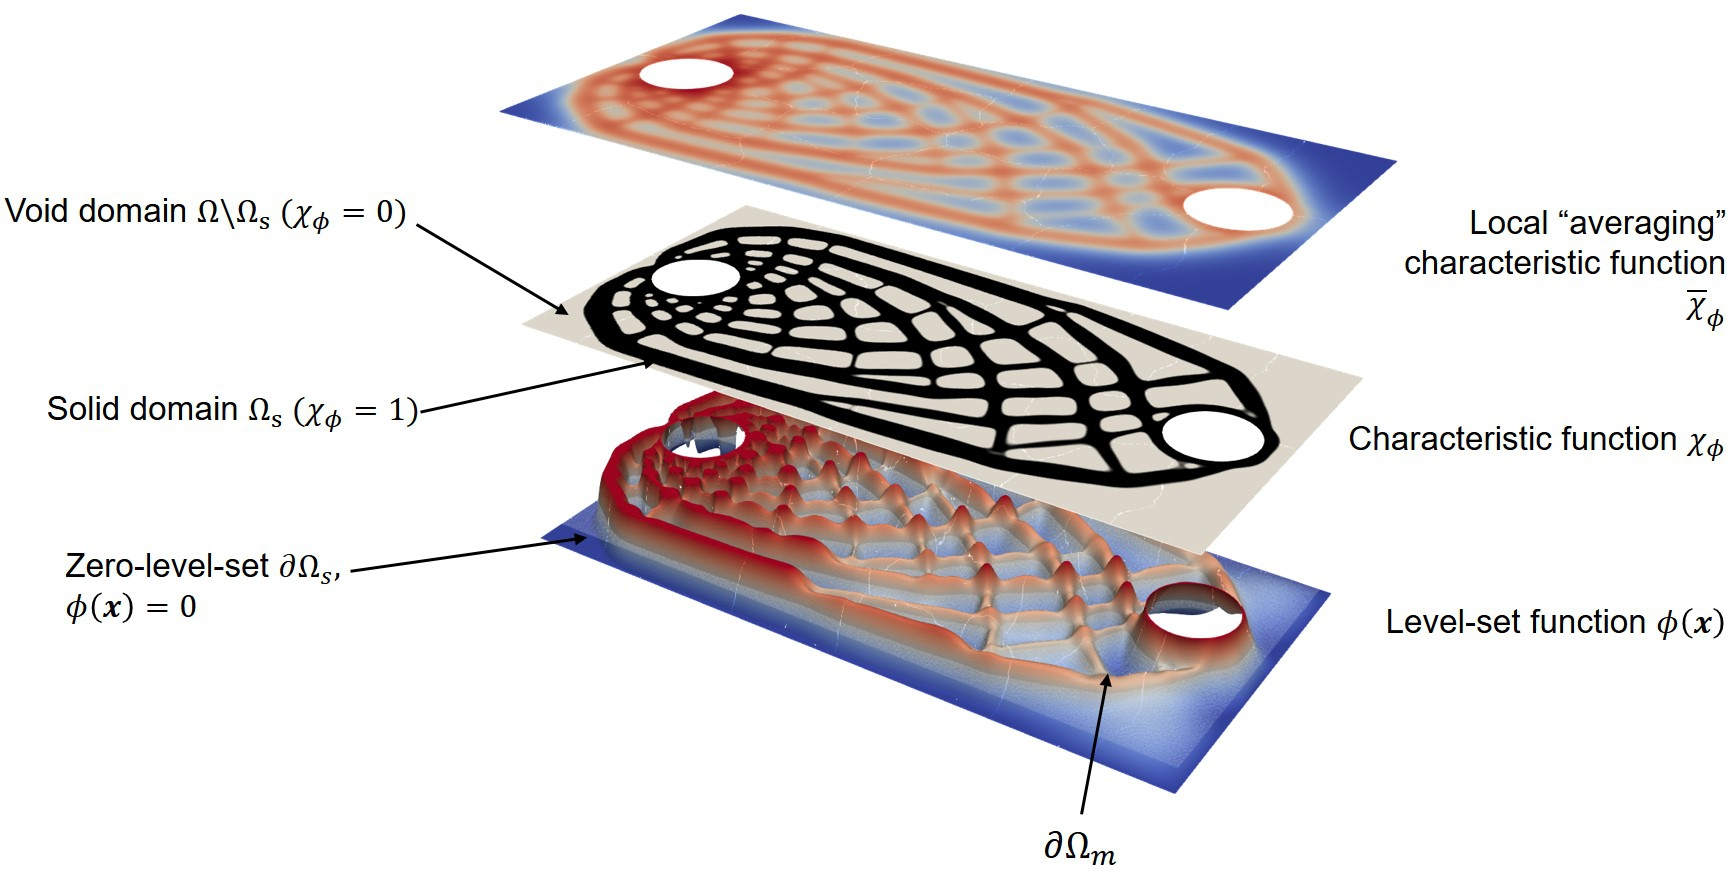
\includegraphics[width=\textwidth]{diagram.jpg}
\caption[Visualization of function used for topology optimization]{Visualization of the level-set ($\phi$), characteristic ($\chi$), and local average characteristic ($\bar{\chi}$) functions for an optimized lattice structure.} \label{fig:infill_diagram}
\end{figure}

\subsection{Optimum design problem for feature-rich structures}\label{Section: topology optimization problem}

The underlying physics of the optimum design problem is the linear elasticity, where the following assumptions are made: (1) small displacements and deformations are observed (linear elasticity), and (2) the body force and gravity are neglected. Furthermore, the context of interest here is to minimize the mean compliance of the structure or, in other words, to maximize the stiffness. Therefore, the topology optimization problem can be formulated as
\begin{subequations}
	\begin{equation}
		\inf _{\chi_{\phi} \in \mathcal{X}} J(\Omega)=\int_{\partial \Omega_{s}^{N}} \boldsymbol{t} \cdot \boldsymbol{u} d \Gamma,
		\label{eq: objective function}
	\end{equation}
	\begin{equation}
		\text { so that }\left\{\begin{array}{ll}
			-\operatorname{div}(\mathbb{C}_{\chi_{\phi}} : e(\boldsymbol{u}))=0 & \text { in } \Omega \\
			\boldsymbol{u}=\boldsymbol{u}_{0} & \text { on } \partial \Omega^{D} \\
			(\mathbb{C}: e(\boldsymbol{u})) \cdot \boldsymbol{n}_{s}=\mathbf{t} & \text { on } \partial \Omega^{N} \\
			G_{1}=\dfrac{\int_{D} \chi d \Omega}{\int_{D} d \Omega}-V_{\max } \leq 0 & \\
			G_2=\left(\dfrac{1}{n} \sum \bar{\chi}^{p}\right)^{1 / p}-\bar{V}_{\max } \leq 0 & \\
			-r^2 \nabla^2 \bar{\chi} +  \bar{\chi} =  \chi & \text{ in } \Omega \\
			\nabla \bar{\chi} \cdot \boldsymbol{n} = 0 & \text{ on } \partial \Omega,
		\end{array}\right.
		\label{eq: governing equation and constraints}
	\end{equation}
	\label{eq: topology optimization mathematical model}
\end{subequations}
where $\Gamma$ is the boundary, $\mathbb{C}$ the fourth-order elasticity tensor, $\boldsymbol{t}$ the surface traction, $e\left(\boldsymbol{u}\right)$ the linearized strain tensor, $\boldsymbol{u}$ displacement, $\boldsymbol{u}_0$ the initial displacement, $\Omega^{D}$ the Dirichlet boundary, $\Omega^{N}$ Neumann boundary, $G_1$ the global volume constraint, and $G_2$ the local volume constraint. Using the characteristic function $\chi_{\phi}$, the elasticity tensor $\mathbb{C}$ can be expanded as
\begin{equation}
	\mathbb{C}_{\chi_{\phi}} = \chi_{\phi} \left(\mathbb{C}_{\text{s}} - \mathbb{C}_{\text{v}} \right) + \mathbb{C}_{\text{v}},
\end{equation}
where $\mathbb{C}_{\text{s}}$ and $\mathbb{C}_{\text{v}}$ are the constitutive tensors for solid and void materials, respectively.

As it is well-known that the mean compliance problem is self-adjoint, the topological design sensitivity can be derived as
\begin{equation}
	\mathcal{F}^{\prime}=-\left(e(\boldsymbol{u}): \mathbb{C}_{\chi_{\phi}}\right): e(\boldsymbol{u})+\lambda_{1} + \lambda_2 \mathcal{G}',
	\label{Eq: design sensitivity}
\end{equation}
where $\lambda_{1}$ and $\lambda_{2}$ are the Lagrange multipliers associated with the global and local averaging volume constraints, respectively. They can be updated using the augmented Lagrange method\ \cite{li2021full}.

The sensitivity associated with the local volume constraint (denoted by $\mathcal{G}'$) is computed as the solution of the following system of equations:
\begin{equation}
	\left\{\begin{aligned}
		& -r^2 \nabla^2 \mathcal{G}' +  \mathcal{G}' =  \dfrac{\partial G_2}{\partial \bar{\chi}} & \text{ in } \Omega \\
		& \nabla\mathcal{G}' \cdot \boldsymbol{n} = 0 & \text{ on } \partial \Omega.
	\end{aligned}\right.
	\label{Eq: G'}
\end{equation}


\end{subappendices}




%%%%%%%%%%%%%%%%%%%%%%%%%%%%%%%%%%%%%%%%%%%%%%%%%%
% Keep the following \cleardoublepage at the end of this file,
% otherwise \includeonly includes empty pages.
\cleardoublepage
